\chapter{Capability Maturity Model Integration}

\section{Introduction}

The \ac{cmmi} model is a model for evaluating the reliability of companies. The model contains guidelines for process improvement within an organization. Since \ac{cmmi}'s inception there are more areas of business the model can be applied to: Production and development (CMMI-DEV), Service establishment (CMMI-SVC) and Product and Service acquisition (CMMI-ACQ)~\citep{ProductCMMIfor2010}.

The \ac{cmmi} model is the successor of the \ac{cmm} model which was developed between 1986 and 1993. The \ac{cmm} model originates from the software development world but is now often used in companies outside of the software business. The \ac{cmm} model was developed by the \ac{sei} by request of the US air force. The US Air force had difficulty finding contractors for their software projects and wanted a way find a way to identify reliable contractors.
% ref for SEI 

\begin{figure}[!ht]
    \centering
        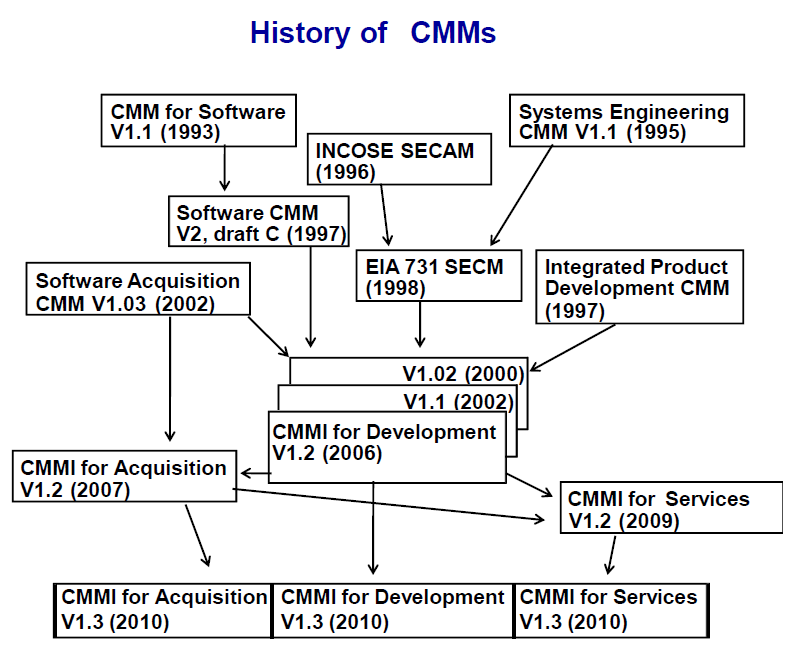
\includegraphics[width=0.6\textwidth]{graphics/cmmi_history}
    \caption{The History of \acp{cmm}}
    \label{fig:cmmi_history}
\end{figure}

\ac{cmmi} is often used when a company's reliability needs to be established, for example, with tender assignments. The \ac{cmmi} model has five levels of maturity an organisation can be assigned, with level five being the highest. \ac{cmmi} does not provide certifications for companies but rather appraises them at one of the five levels of \ac{cmmi}. Companies are often appraised when they accept new contracts or when they want to measure how their production process is working compared to \ac{cmmi} best practices. If an organisation wants to increase its \ac{cmmi} maturity level this can take between five to twenty months.%Citation needed!

\section{The \acs{cmmi} model framework}
% Needs REF.
The \ac{cmmi} model framework consist of the following core process areas:
%JWD: made more compact.
\begin{compactitem}
    \item \ac{car}
    \item \ac{cm}
    \item \ac{dar}
    \item \ac{ipm}
    \item \ac{ma}
    \item \ac{opd}
    \item \ac{opf}
    \item \ac{opm}
    \item \ac{opp}
    \item \ac{ot}
    \item \ac{pi}
    \item \ac{pmc}
    \item \ac{pp}
    \item \ac{ppqa}
    \item \ac{qpm}
    \item \ac{rd}
    \item \ac{reqm}
    \item \ac{rskm}
    \item \ac{sam}
    \item \ac{ts}
    \item \ac{val}
    \item \ac{ver}
\end{compactitem}

\section{Competence Areas in the Processes}
The \ac{scrum}, \ac{rup} and the process followed by Ariane 5 will be judged on how well the core process areas are covered by these processes. 
This is done in table~\ref{tab:cmmi_l2} for level two, table~\ref{tab:cmmi_l3} for level three, table~\ref{tab:cmmi_l4} for level four, and table~\ref{tab:cmmi_l5} for level five.

The following coverage levels are assigned to each process area for each process.
\begin{compactdesc}
\item[High] Fully covered by process used.
\item[Medium] Partially covered by process used.
\item[Low] Poorly covered by process used.
\item[None] Not covered by process used.
\item[Unknown] Not enough information to determine level.
\end{compactdesc}
% Plan:
% - Set criteria to determine if competency applies to process

\begin{table}[ht!]
    \centering
    \begin{tabular}{>{\bfseries}l|*{7}{c}}
        Process     & \acs{cm} & \acs{ma} & \acs{pmc} & \acs{pp} & \acs{ppqa} & \acs{reqm} & \acs{sam}  \\
        \toprule
        RUP         & High & Medium & Medium & Medium & High & High & None \\ 
        Scrum       & Low & High & High & High & Low & High & None \\ 
        Ariane 5    & Unknown & Low & Unknown & Low & Unknown & Unknown & Unknown \\ 
    \end{tabular}
    \caption{Maturity Level 2 - Managed}
    \label{tab:cmmi_l2}
\end{table}


\begin{table}[ht!]
    \centering
    \begin{tabular}{>{\bfseries}l|*{6}{c}}
        Process & \acs{dar} & \acs{ipm} & \acs{opd} & \acs{opf} & \acs{ot} & \acs{rskm} \\
        \toprule
        RUP     & None & Medium & None & None & None & Medium \\
        Scrum   & None & Medium & Low & Medium & None & Low \\ 
        Ariane 5 & Unknown & High & Unknown & Unknown & Unknown & Medium \\
    \end{tabular}
    \vspace{\baselineskip}\linebreak
    \begin{tabular}{>{\bfseries}l|*{5}{c}}
         Process & \acs{rd} & \acs{ts} & \acs{pi} & \acs{ver} & \acs{val} \\
         \toprule
         RUP & High & Medium & High & High & High \\ 
         Scrum & High & None & None & None & None \\ 
         Ariane 5 & - & - & - & - & - \\ 
    \end{tabular}
    \caption{Maturity Level 3 - Defined}
    \label{tab:cmmi_l3}
\end{table}

\begin{table}[ht!]
    \centering
    \begin{tabular}{>{\bfseries}l|cc}
        Process & \acs{opp} & \acs{qpm} \\
        \toprule
        RUP     & None & Low \\   
        Scrum   & - & - \\
        Ariane 5 & Unknown & Unknown \\
    \end{tabular}
    \caption{Maturity Level 4 - Quantitatively Managed}
    \label{tab:cmmi_l4}
\end{table}

\begin{table}[ht!]
    \centering
    \begin{tabular}{>{\bfseries}l|cc}
        Process & \acs{car} & \acs{opm} \\
        \toprule
        RUP     & Low & None \\
        Scrum   & - & - \\
        Ariane 5 & High & Unknown \\
    \end{tabular}
    \caption{Maturity Level 5 - Optimising}
    \label{tab:cmmi_l5}
\end{table}


\FloatBarrier

\subsection{RUP \& CMMI}

As it is mentioned in the '\ac{cmmi} for developers' document~\citep{team2010cmmi}, \ac{cmmi} itself is not a process description, but instead it describes characteristics (process areas) of a good software process. Additionally, it is a map that identifies gaps in existing processes that may need to be filled. 
On the other hand, \ac{rup} is an iterative software process which maps to many \ac{cmmi} process areas. 
While \ac{cmmi} describes the ``what'', \ac{rup} describes the ``how''. 
The synergy between those two addresses any gaps they collectively define and eliminates redundancy. 
As it can be seen from the table and as Gallagher et al.~\citep{gallagher2001rational} conclude; \ac{rup} maps some parts \ac{cmmi} in it's workflows and activities.

\subsubsection{Maturity Level 2}
First, analysing the \textbf{\textit{Maturity Level 2}} process area, "\ac{cm} is present in \ac{rup} as a specific artifact, including an established \ac{cm} system, tracking and controlling changes, and configuration audits.

\ac{ma} is not defined explicitly in \ac{rup}; there is no description on details or metrics and analytics definition. However, the definition includes measurements specification, analysis reports, results and communicative data.

\ac{pmc} in \ac{rup} has some some incompatibilities, while \ac{rup} monitors areas such as project planning, risks, stakeholders, progress and milestones, it has problems on commitments monitoring and data management. Also, \ac{rup}'s corrective actions are explicit and include issues management and corrective actions management.

Furthermore, \ac{pp} is slightly supported by \ac{rup} since it includes definitions of the project size, efforts and cost estimation and risks identification. But it does not support project attributes estimation, data management and project resources planning. 

\ac{ppqa} is mapped by \ac{rup} owning to the support of evaluation of the processes, products and services.
The mapping of \ac{reqm} and \ac{rup} is also clear because in \ac{rup} the inception phase is consisted of a set of requirements analysis including commitment, support of changes and support of later requirements refinements. 

Last element of this process area is the \ac{sam}. \ac{rup} has no support on this area since it is not defined at all.

\subsubsection{Maturity Level 3}
Second, in case of the \textbf{\textit{Maturity Level 3}} process area.

\ac{dar}, \ac{opd}, \ac{opf}, \ac{ot} are not defined in \ac{rup} and are not supported inside the scope of \ac{rup}. However, \ac{ipm} has a few points which can be mapped in \ac{rup}, including the integrated plans in project management, issues resolving and stakeholders involvement management. In addition to that, \ac{rup} slightly supports integrated plans and project process establishment but no dependencies management.

\ac{rup} is a risk-first process by including risk identification, classification and prioritisation has not clear definition for risk management strategies \ac{rskm}.

The development, validation and analysis of the requirements \ac{rd} in \ac{rup} is very explicit process. From the customer perspective, during the inception phase, there is requirements elicitation, stakeholders needs collection and  transformation from stakeholders needs to customer requirements. On the product requirements side, there is explicit product establishment identification.

\ac{ts} addressed by \ac{rup} in many different levels. First, the selection of product component solutions is missing from \ac{rup} since it is not mentioned a detailed alternative solutions development, but the evolution of operational concepts and scenarios are clear. Next, \ac{rup} is very specific in development and design, it suggests effective design methods, comprehensive interfaces and interfaces descriptions establishment.

% TODO: Product Integration
\ac{pi} in \ac{rup} is established by \textit{product integration strategies} and \textit{environments}, interfaces management, and finally, explicit component integration and product deployment procedures.

Both \ac{ver} and \ac{val} are established by specific practises of \ac{rup}. First, \ac{rup} for verification, it includes a verification strategy and environment, including peer reviews and analyses of review data. Second, for validation, it also includes validation strategy and environment. Additionally for both cases data gathering and analysis is included for continuous improvement.

\subsubsection{Maturity Level 4}
Third, \textbf{\textit{Maturity Level 4}} process area includes \ac{opp} which is not defined in the scope of \ac{rup} and \ac{qpm} which is it can be slightly mapped in the composition of the defined process that \ac{rup} supports.

\subsubsection{Maturity Level 5}
Finally, in \textbf{\textit{Maturity Level 5}} process area \ac{car} can slightly mapped in \ac{rup} in terms of analysis data selection support and changes evaluation. 
However, \ac{opm} is something that is not mentioned in \ac{rup}.

\subsection{Scrum \& CMMI}
\subsubsection{Maturity Level 2}
When we dive into analysing \textbf{\textit{Maturity Level 2}} for the Scrum framework we are able to conclude that a lot of process areas are well covered. 

However, if we look into \ac{cm} area it is easy to point out that Scrum is not always that specific. In fact, for \ac{cm} only the User Stories are described by Scrum. 

Furthermore, it is easy to conclude that \ac{ma} is highly covered within Scrum. Simply put, the Scrum Master has the sole responsibility to maintain the Scrum framework implementation itself \citep{schwaber2011scrum}. 

The \ac{pmc} is also recognised as a strong area in Scrum. As the framework is concentrated in delivery, Scrum includes useful practises for project monitoring and control. Moreover, Scrum integrates the Sprint Planning, Daily Scrum, Sprint, Sprint Review and the Sprint Retrospective in order to accomplish successful control over the work, and monitoring over the separate development steps. Furthermore, the Sprint Planning and the Sprint Review are collaborating highly for the success in the \ac{pp} area. 

In addition, the Product Owner role is responsible for interacting with relevant stakeholders appropriately, and giving guidance to the Development Team in terms of business requirements. However, Scrum is not very specific about quality assurance. The Definition of "Done" is agreed within the team and the process itself is not definite enough about the \ac{ppqa}. 

Since all the business requirements are covered specifically by the Product Owner, Scrum has a dedicated role. Therefore the \ac{reqm} area is also well covered. 

Last but not least, \ac{sam} is not described in Scrum.

\subsubsection{Maturity Level 3}
In contrast to the previous level, \textbf{\textit{Maturity Level 3}} is not so well defined within the \ac{scrum} framework. Process areas such as \ac{dar}, \ac{ot}, \ac{ts}, \ac{pi}, \ac{ver} and \ac{val} are not described in \ac{scrum}.

However, the \ac{rd} area is implemented within the Scrum framework with the usage of Sprint Planning meetings, Sprint Reviews and Sprint Retrospectives.

Furthermore, the \ac{ipm} is expressed in \ac{scrum} by the Increment \citep{schwaber2011scrum}, the Scrum Retrospective, and the Scrum of Scrums \citep{sutherland2001inventing}. Simply put, the Increment can be used to estimate time-frames better, the Scrum Retrospective to learn from mistakes made during the Sprint and the Scrum of Scrums to spread lessons throughout the entire organization. The Scrum Retrospective and the Scrum of Scrums also collaborate for having a medium state of \ac{opf}. The Scrum of Scrums in particular also gives the framework a glimpse of what \ac{opd} is.

Finally, we have the \ac{rskm} which is not specifically expressed within Scrum. As Scrum is focused generally on product delivery, the risk management is limited only to technical risks. In fact, even the technical risk management is dependant on the definition of "Done" \citep{schwaber2011scrum}.


\subsection{Ariane 5 \& CMMI}
This subsection is meant to analyse the failed case we chose during Assignment 1 of the Software Process course.
We will be assessing to what extent the organisational process for the development of the Ariane 5 rocket fits the \ac{cmmi} model. 
%maybe put this as a footnote or smth?
It should be noted that, similar to Assignment 1, the amount of information available concerning the Ariane 5 development process is scarce.

\subsubsection{Maturity Level 2}
We begin with assessing compliance to \textbf{\textit{Maturity Level 2}}. We know that the process is spread across a multitude of companies. This would indicate that there has to be some form of \ac{cm} in order to manage code configurations and releases. However actual information concerning \ac{cm} in the Ariane 5 development process is \textit{unknown} to us. 

\ac{ma} assess the compliance of an organisations' process in order to quantify aspects that belong to it. In terms of software development this would equal to testing and software metrics. What we know from the Ariane case is that one of the problems that was identified concerned inadequate testing. Information concerning software metrics is \textit{unknown} to us. This would mean that compliance with \ac{ma} is \textit{low} at best. 

Compliance to \ac{pmc} is \textit{unknown} to us. 

Concerning compliance to \ac{ppqa}, we have certain documents showing evaluations of tools/methodologies used during the development process. For example we know that the programming language Ada had specific pitfalls developing for certain targets (processors). These evaluations were largely ignored. Considering this information we would assess compliance as \textit{low}. However as we do not have any information concerning the  processes in place, we will state that compliance to \ac{ppqa} is \textit{unknown} to us. 

Compliance to \ac{reqm} is \textit{unknown} to us. 

Compliance to \ac{sam} is \textit{unknown} to us. We do have information concerning the amount of prime-contractors and sub-contractors for the Ariane case. Though information on how the suppliers are managed is not known.

\subsubsection{Maturity Level 3}
Compliance to \textbf{\textit{Maturity Level 3}} is described below.
We have insufficient information to assess compliance to \ac{dar}. We do know that decisions were made about a testing vs. performance trade-off consistently. However, these are undocumented in the shape of a formal decision making process. We conclude that the compliance is \textit{unknown} despite this information. 

Compliance to \ac{ipm} is \textit{high}. We know that \ac{esa} had defined a multitude of processes for project management. These were established as early as 1982 when \ac{esa} commissioned the HOOD methodology for managing software within the project. 

Compliance to \ac{opd} is \textit{unknown} to us. Information we do have suggests usage of a Waterfall-esque method. Compliance to \ac{opf} is \textit{unknown} to us. 

Compliance to \ac{ot} during the time our case was relevant is \textit{unknown}. According to \citep{esatraining2016} \ac{esa} currently does offer training programmes. 

Compliance to \ac{rskm} we assess as \textit{medium}. This is due to papers/articles such as \citep{nuseibeh1997ariane}. Where they state that inadequate risk-management played a significant role in the failure of the case.

\subsubsection{Maturity Level 4}
Compliance to \textbf{\textit{Maturity Level 4}} is described below. 

Compliance to \ac{opp} is \textit{unknown} to us. In our research for this case we were unable to find any quantitative assessments performed by the organization themselves before the failure. 

Compliance to \ac{qpm} at the moment of failure is \textit{unknown} to us. Currently is it known to us that \ac{esa} has developed a project management tool that addresses/quantifies project management \citep{esapmgmnt2016}.

\subsubsection{Maturity Level 5}
Compliance to \textbf{\textit{Maturity Level 5}} is described below. 

Compliance to \ac{car} is \textit{high}. In the Ariane case extensive research has been done in order to learn as much as possible from the failure and prevent future failures. 

Compliance to \ac{opm} is \textit{unknown} to us. We have found several examples where \ac{esa} requests feedback to improve performance. Though these are current day examples. Concerning the time-period of the failure little information is available.

\section{Planning \& Predictability in Scrum \& RUP}
%% Potentially split up later, based on analysis in table.
%% Reason both ways in the analysis: why would RUP trump Scrum and why would Scrum trump RUP?

\section{Conclusion}
%% Valuable lessons from this section go here.
\subsection{Ariane 5}
%Only thing I really learned is that the Ariane case had lots of pitfalls
% I think that a compliance with CMMI especially the evalutation/improvement part would have helped ESA a lot because I found reports from people who worked on the OBC
%They said that they had to trade-off testing for performance
%Which they would have found if they had done something with the reports
